\chapter{Background}
\label{cp:Background}

\begin{comment}
Please write down the basic background for your research, e.g., the fundamental concepts of the approaches that you use in the thesis, so that other people (who do not have the background) can understand your work.

Here is one example for sigmoid function:

The sigmoid function is defined by formula~\ref{eq:sigmoid}. It can compress the input into the interval $(0, 1)$. The drawback of the sigmoid activation function is the so-called ``kill gradients'': if the input values locate in the tail of 0 or 1, the gradient at these regions tend to be zero. If the sigmoid function is used multiple times in a neural network, the gradients may be very small or even disappear.

\begin{equation}
\label{eq:sigmoid}
\centering{f(x) = \frac{1}{1 + e^{-x}}}.
\end{equation}
\end{comment}

\section{Discrete wavelet decomposition}

The foundations of the Discrete wavelet transform (DWT) go back to 1976 when Croiser, Esteban, and Galand devised a technique to decompose discrete time signals. Crochiere, Weber, and Flanagan did a similar work on coding of speech signals in the same year. They named their analysis scheme as subband coding. In 1983, Burt defined a technique very similar to subband coding and named it pyramidal coding which is also known as multiresolution analysis. Later in 1989, Vetterli and Le Gall made some improvements to the subband coding scheme, removing the existing redundancy in the pyramidal coding scheme.~\cite{polikar1996wavelet}.

DWT is any wavelet transform for which the wavelets are discretely sampled. As with other wavelet transforms, a key advantage it has over Fourier transforms (FT) is temporal resolution: it captures both frequency and location information (location in time). 

In Fourier transforms we cannot know what spectral component exists at any given time instant. The best we can do is to investigate what spectral components exist at any given interval of time. This is a problem of resolution, and it is the main reason why we use wavelet transform (WT) instead FT. FT gives a fixed resolution at all times, whereas WT gives a variable resolution as follows:

Higher frequencies are better resolved in time, and lower frequencies are better resolved in frequency. This means that, a certain high frequency component can be located better in time domain (with less relative error) than a low frequency component. On the contrary, a low frequency component can be located better in frequency domain compared to high frequency component.

we can visualize the resolution problem at figure ~\ref{fig:resolution}:

\begin{figure}[h]
\centering
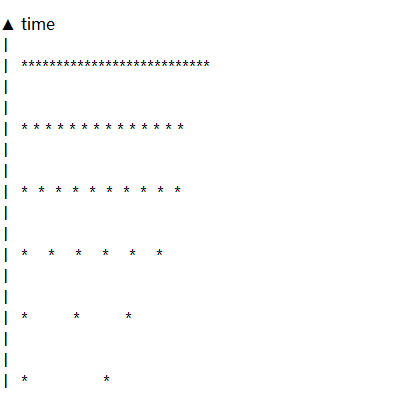
\includegraphics[width=1\textwidth]{images/resolution_blank1.PNG}
\caption{high frequency signal is better resolved in time domain}
\label{fig:resolution}
\end{figure}



\begin{figure}[h]
\centering
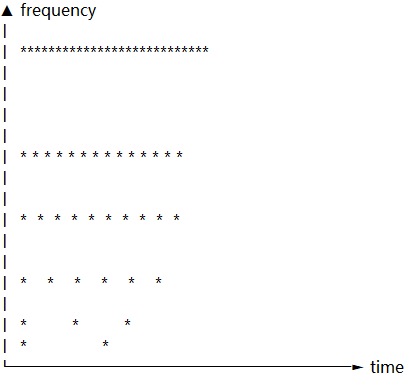
\includegraphics[width=1\textwidth]{images/resolution_blank2.PNG}
\caption{low frequency signal is better resolved in frequency domain}
\label{fig:resolution_frequency}
\end{figure}

In figure ~\ref{fig:resolution} the top row shows that at higher frequencies we have more samples corresponding to smaller intervals of time. In other words, higher frequencies can be resolved better in time, which mean we can easily find out higher frequency signal in time domain. As the frequency decrease there are less number of points to characterize the signal, therefore, low frequencies have poor resolution in time domain. 

In figure ~\ref{fig:resolution_frequency}, the time resolution of the signal works the same as show in figure ~\ref{fig:resolution}, but now, the frequency information has different resolutions at every stage too. We can note that the space between subsequent frequency components increase as frequency increases. Thus lower frequencies are better resolved in frequency, where as higher frequencies are not.

multiresolution analysis (MRA), also known as Discrete wavelet transform, is a framework proposed to analyzes the signal at different frequencies with different resolutions. MRA is designed to give good time resolution at high frequencies as well as good frequency resolution at low frequencies. This approach makes sense especially when the signal at hand has high frequency components for short durations and low frequency components for long durations. Fortunately, the most signals that are encountered in practical applications are often of this type.

The DWT procedure starts with passing the discrete signal $x[n]$ through a half band digital lowpass filter with impulse response h[n]. Filtering a signal corresponds to the mathematical operation of convolution of the signal with the impulse response of the filter. The convolution operation in discrete time is defined as follows:

\begin{equation}
y[n]=x[n] * h[n]=\sum_{k=-\infty}^{\infty} x[k] \cdot h[n-k]
\label{equ:convolude}
\end{equation}

After passing the signal through a half band lowpass filter, Signals with frequencies larger than f/2 have disappeared. Since half the frequencies of the signal have now been removed, half the samples can be discarded according to Nyquist’s rule. This can be achieved by subsampling the singal by two, and the signal will then have half the number of points. The resolution of this signal, which is a measure of the amount of detail information in the signal, is halved by the lowpass filter operation. While the scale, which is the inverse of frequency, of the signal is now doubled. 

In order to better illustrate the parameter scale, we can image it as the scale used in maps: high scales in case of map correspond to a non-detailed global view (of the signal), and low scales correspond to a detailed local view. Similarly, in terms of frequency, low frequencies (high scales) correspond to a global information of a signal (that usually spans the entire signal), whereas high frequencies (low scales) correspond to a detailed information of a hidden pattern in the signal. 

One thing worth paying special attention to is that the subsampling operation after filtering does not affect the resolution, since removing half of the spectral components from the signal (in which the number of sample stay unchanged) makes half the number of samples redundant anyway. Thus, half the samples can be discarded without any loss of information. In summary, the lowpass filtering halves the resolution, but leaves the scale unchanged. The signal is then subsampled by two since half of the number of samples are redundant. This doubles the scale.

This procedure can mathematically be expressed as

\begin{equation}
y[n]=\sum_{k=-\infty}^{\infty} x[k] \cdot h[2 n-k]
\label{equ:subband}
\end{equation}

For the principle of decomposes the signal with DWT, we can draw the following conclusions: The DWT analyzes the signal at different frequency bands with different resolutions by decomposing the signal, which is achieved by filtering the time domain signal successively with highpass and lowpass. The signal filtered by highpass and lowpass constitutes one level of decomposition and can
mathematically be expressed as follows:

\begin{equation}
\begin{aligned}
&y_{\text {low }}[n]=\sum_{k=-\infty}^{\infty} x[k] g[2 n-k] \\
&y_{\text {high }}[n]=\sum_{k=-\infty}^{\infty} x[k] h[2 n-k]
\end{aligned}
\end{equation}

where $y_{\text {high }}[n]$ and $y_{\text {low }}[n]$ are the outputs of the highpass and lowpass filters after subsampling by two, respectively, which correspond to detail information and coarse approximation.

After decomposition, the time resolution of signal is halved, while the frequency resolution is doubled, this is because only half of the number of samples can represent the entire signal, and the frequency band of the signal only spans half of the previous frequency band. The above process is also called subband coding, and can be repeated for further decomposition. At each level, filtering and subsampling will cause the number of samples to be halved (thus the time resolution is halved) and the spanned frequency band is halved (thus the frequency resolution is doubled). This procedure is shown in Figure ~\ref{fig:dwt1}, in which x[n] is the original signal, and h[n] and g[n]
are lowpass and highpass filters, respectively. f represent the band width of each level. 

\begin{figure}[h]
\centering
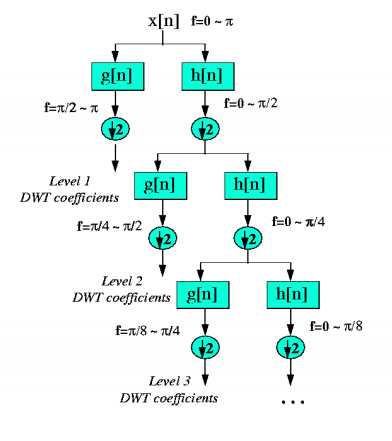
\includegraphics[width=1\textwidth]{images/dwt1.PNG}
\caption{the DWT decomposition algorithms}
\label{fig:dwt1}
\end{figure}














\section{Control chart}



Statistical process control (SPC) is a powerful collection of problem-solving
tools useful in achieving process stability and improving capability through the reduction of variability.
SPC is one of the greatest technological developments of the twentieth century because it is based on sound underlying principles, is easy to use, has significant impact, and can be applied to any process~\cite{montgomery2020introduction}. Its seven major tools are
\begin{enumerate}
    \item Histogram or stem-and-leaf plot
    \item Check sheet
    \item Pareto chart
    \item Cause-and-effect diagram
    \item Defect concentration diagram
    \item Scatter diagram
    \item Control chart
\end{enumerate}

Of this seven tools, Control chart is probably the easiest yet effective tool to analyze the process stability. To best understand the concepts of Control chart, the classification of Control chart need to be clarified. Depending on the number of process characteristics to be monitored, there are two basic types of control charts. The first, referred to as a univariate control chart, is a graphical chart of one quality characteristic, in which one is interested in monitoring changes in the parameter of an underlying univariate distribution
over time. The second is a multivariate control chart, which is a graphical chart of a statistic that fuses more than one quality characteristic to monitor simultaneous changes in the parameter
vector of an underlying multivariate distribution over time.


More specificlly, the control chart is a graphical display, which plots the value of the quality characteristic that has been measured or calculated from a sample versus the sample number or versus time. Normally there are three lines in a control chart: a center line that correspond to the mean value for the in-control process. Two other horizontal lines, called the upper control limit (UCL) and the lower control limit (LCL). These control limits are chosen so that almost all of the data points will fall within these limits as long as the process remains in-control. A typical control chart is shown in Fig.~\ref{fig:control_chart}.

\begin{figure}[h]
\centering
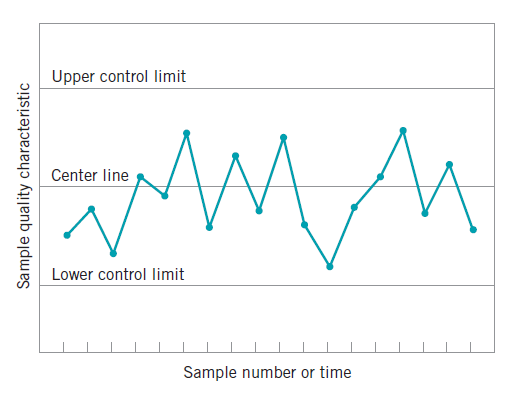
\includegraphics[width=1\textwidth]{images/control_chart.PNG}
\caption[A typical control chart.]{a center line that correspond to the mean value for the in-control process. Two other horizontal lines, called the upper control limit (UCL) and the lower control limit (LCL). Figure is adapted from ~\cite{montgomery2020introduction}}
\label{fig:control_chart}
\end{figure}

\subsection{Shewhart $\bar{X}$ control chart}
In statistical quality control, the $\bar{X}$ and s chart is a type of control chart used to monitor variables data when samples are collected at regular intervals from a business or industrial process ~\cite{heckert2002handbook}. 

In general, $\bar{X}$ and s control chart has following advantages:
\begin{enumerate}
    \item The sample size (n) is relatively large $(n>10)$.
    \item The sample size is variable.
\end{enumerate}

The chart actually consists of two individual control charts: One ($\bar{X}$ control chart) to monitor the process mean and the other (s control chart) to monitor the process standard deviation.

During the 1920's, Dr. Walter A. Shewhart proposed a general model for control charts as follows :

Let s be a sample statistic that measures some continuously varying quality characteristic of interest (e.g., diameter), and suppose that the mean of s is $\mu_{s}$, with a standard deviation of $\sigma_{s}$. Then the center line (CL), the upper control limit (UCL), and the lower control limit (LCL) are


\begin{equation}
    U C L=\mu_{s}+k \sigma_{s}
    \label{equ:UCL}
\end{equation}

\begin{equation}
    C L=\mu_{s}
    \label{equ:CL}
\end{equation}

\begin{equation}
    U C L=\mu_{s}-k \sigma_{s}
    \label{equ:LCL}
\end{equation}

where k is the distance of the control limits from the center line, expressed in terms of standard deviation units. When k is set to 3, we speak of 3-sigma control charts. Historically, k=3 has become an accepted standard in industry.

The centerline is the process mean, which in general is unknown, so as the $\sigma$. We need to replace them with some confident values. e.g., the average of all the data and the average standard deviation, respectively. 

There exit two distinct phases of the control chart
~\cite{bersimis2007multivariate}:

\begin{itemize}
\item Phase I: charts are used for retrospectively testing whether the process was in control when the first
subgroups were being drawn. In this phase, the charts are used as aids to the practitioner, in bringing a
process into a state where it is statistically in control.
\item Phase II: control charts are used for testing whether the process remains in control when future subgroups
are drawn. In this phase, the charts are used as aids to the practitioner in monitoring the process for any
change from an in-control state.
\end{itemize}

In short, phase I that deals with estimating process parameters to ensure process stability using historical data, and phase II pertains to signal
any out‐of‐control condition or shifts in the process parameters.

Suppose in phase I we have m samples at our disposition, and let $d_{i}$ be the parameter (s) of the i-th sample. Then the average of the parameter is


\begin{equation}
    \mu_{s}=\frac{1}{m} \sum_{i=1}^{m} d_{i}
    \label{equ:mu}
\end{equation}

If $\sigma^{2}$ is the unknown variance of a probability distribution, then an unbiased estimator of $\sigma^{2}$ is the sample variance is

\begin{equation}
    s^{2}=\frac{\sum_{i=1}^{m}\left(d_{i}-\bar{x}\right)^{2}}{m-1}
    \label{equ:sigma}
\end{equation}

However, s, the sample standard deviation, is not an unbiased estimator of $\sigma$. If the underlying distribution is normal, then s is actually

\begin{equation}
    s=c_4 \times \sigma
    \label{equ:s}
\end{equation}

where $c_4$ is 

\begin{equation}
    c_{4}=\sqrt{\frac{2}{m-1}} \frac{\left(\frac{m}{2}-1\right) !}{\left(\frac{m-1}{2}-1\right) !}
    \label{equ:c4}
\end{equation}

in which m is the sample size.

Finally, the standard deviation of the sample standard deviation is

\begin{equation}
    \sigma_{s}=\sigma \sqrt{1-c_{4}^{2}}
    \label{equ:sigma_s}
\end{equation}

\subsection{Hotelling $T^{2}$ control chart}
In fact the most data in industry (especially In the field of chemistry and manufacturing)are naturally multivariate. Hotelling in 1947 introduced a statistic which uniquely lends itself to plotting multivariate observations. This statistic, appropriately named Hotelling's  $T^{2}$, is a scalar that combines information from the mean of several variables. We can image this scalar (so-called Hotelling $T^{2}$ distance) as a statistic describing the distance away from Mean. The derivation of Hotelling $T^{2}$ distance is as follows:

%\subsubsection{Multivariate normal distribution}
In univariate statistical quality control, we generally use the normal distribution to describe the behavior of a continuous quality characteristic. The univariate normal probability density function is


\begin{equation}
    f(x)=\frac{1}{\sqrt{2 \pi \sigma^{2}}} e^{-\frac{1}{2}\left(\frac{x-\mu}{\sigma}\right)^{2}} \quad-\infty<x<\infty
    \label{equ:normal_distribution}
\end{equation}

The mean of the normal distribution is $\mu$ and the variance is $\sigma$. The term (apart from the minus sign) in the exponent of the normal distribution can be written as follows:

\begin{equation}
    (x-\mu)\left(\sigma^{2}\right)^{-1}(x-\mu)
    \label{equ:normal_distribution_part}
\end{equation}

This quantity measures the squared standardized distance from x to the mean $\mu$, where by the term “standardized” we mean that the distance is expressed in standard deviation units. This same approach can be employed in the multivariate normal distribution case. 

Suppose we have p variables, given by $x_{1}, x_{2}, \ldots, x_{p}$. These variables are arranged in a p-component vector $\mathbf{x}^{\prime}=\left[x_{1}, x_{2}, \ldots, x_{p}\right]$. Let $\mu^{\prime}=\left[\mu_{1}, \mu_{2}, \ldots, \mu_{p}\right]$ be the vector of the means of the x’s, and let the variances and covariances of the random variables in $\mathbf{X}$ be contained in a $p × p$ covariance matrix $\Sigma$. The main diagonal elements of $\Sigma$ are the variances of the x’s and the off-diagonal elements are the covariances. Now the squared standardized distance from $\mathbf{x}$ to $\mu$ is

\begin{equation}
    (\mathbf{x}-\mu)^{\prime} \Sigma^{-1}(\mathbf{x}-\mu)
    \label{equ:squared standardized (generalized) distance}
\end{equation}

Since we extend the concept of mu and sigma from univariate parameter into multivariate parameters, then our next step is naturally to figure out how to construct sample mean vector ($\overline{\mathbf{x}}$) and sample covariance matrix ($\mathbf{S}$) so that they can achieve the same effect as Shewhart $\bar{X}$ control chart.

Suppose that we have a random sample from a multivariate normal distribution
\begin{equation}
\mathbf{x}_{1}, \mathbf{x}_{2}, \ldots, \mathbf{x}_{n}
\label{equ:x1_xn}
\end{equation}

where the ith sample vector contains observations on each of the p variables 
$x_{i 1}, x_{i 2}, \ldots, x_{i p}$. Then the sample mean vector ($\overline{\mathbf{x}}$) is

\begin{equation}
\overline{\mathbf{x}}=\frac{1}{n} \sum_{i=1}^{n} \mathbf{x}_{i}
\label{equ:x_mean}
\end{equation}

and the sample covariance matrix ($\mathbf{S}$) is

\begin{equation}
\mathbf{S}=\frac{1}{n-1} \sum_{i=1}^{n}\left(\mathbf{x}_{i}-\overline{\mathbf{x}}\right)\left(\mathbf{x}_{i}-\overline{\mathbf{x}}\right)^{\prime}
\label{equ:S_x}
\end{equation}

That is, the sample variances on the main diagonal of the matrix S are computed as

\begin{equation}
s_{j}^{2}=\frac{1}{n-1} \sum_{i=1}^{n}\left(x_{i j}-\bar{x}_{j}\right)^{2}
\label{equ:S_j}
\end{equation}

and the sample covariances are

\begin{equation}
s_{j k}=\frac{1}{n-1} \sum_{i=1}^{n}\left(x_{i j}-\bar{x}_{j}\right)\left(x_{i k}-\bar{x}_{k}\right)
\label{equ:S_ij}
\end{equation}

Now suppose that $\mathbf{S}$ from equation (~\ref{equ:S_x}) is used to estimate
$\Sigma$ and that the vector ${\overline{\mathbf{X}}}$ is taken as the in-control value of the mean vector of the process. The Hotelling $T^{2}$ statistic is

\begin{equation}
T^{2}=n(\overline{\mathbf{x}}-\overline{\overline{\mathbf{x}}})^{\prime} \mathbf{S}^{-1}(\overline{\mathbf{x}}-\overline{\overline{\mathbf{x}}})
\label{equ:T2_n}
\end{equation}

in which n is the subgroup size of each sample.

In some industrial settings (e.g., chemical and process industries) the subgroup size is naturally $n = 1$. Then the Hotelling $T^{2}$ statistic in equation
(~\ref{equ:T2_n}) becomes

\begin{equation}
T^{2}=(\overline{\mathbf{x}}-\overline{\overline{\mathbf{x}}})^{\prime} \mathbf{S}^{-1}(\overline{\mathbf{x}}-\overline{\overline{\mathbf{x}}})
\label{equ:T2}
\end{equation}

The phase II control limits for this statistic are
\begin{equation}
\begin{aligned}
\centering&\text { UCL }=\frac{p(m+1)(m-1)}{m^{2}-m p} F_{\alpha, p, m-p} \\
\centering&\text { LCL }=0
\end{aligned}
\end{equation}









































\begin{comment}
Firstly, let's consider the s chart, which is employed to determine if the distribution for the process characteristic is stable.
Suppose we have m preliminary samples at our disposition, each of size n, and let $s_i$ be the standard deviation of the ith sample. Then the average of the m standard deviations ($\bar{s}$) is
\begin{equation}
    \bar{s}=\frac{1}{m} \sum_{i=1}^{m} s_{i}
    \label{equ:s}
\end{equation}
\end{comment}




















